
% This LaTeX was auto-generated from MATLAB code.
% To make changes, update the MATLAB code and republish this document.

\documentclass{article}
\usepackage{graphicx}
\usepackage{color}

\sloppy
\definecolor{lightgray}{gray}{0.5}
\setlength{\parindent}{0pt}

\begin{document}

    
    \begin{verbatim}
% Name - Surag P
% Roll No. - 181EC248

% Experimment Eight

%Simulate PCM and demodulation system and plot the waveforms.

clear
clc

%Sample Sequence
bits = [1 0 1 0 0 0 1 1 0]
bitrate = 1;
figure;

%Unipolar Non-Return Zero
[t,s] = unrz(bits,bitrate);
subplot(5,1,1)
plot(t,s,'LineWidth',1.5);
axis([0 t(end) -0.1 1.1])
grid on;
title('Unipolar NRZ');

%Unipolar Return Zero
[t,s] = urz(bits,bitrate);
subplot(5,1,2)
plot(t,s,'LineWidth',1.5);
axis([0 t(end) -0.1 1.1])
grid on;
title('Unipolar RZ');

%Polar Return Zero
[t,s] = prz(bits,bitrate);
subplot(5,1,3)
plot(t,s,'LineWidth',1.5);
axis([0 t(end) -1.1 1.1])
grid on;
title('Polar RZ');

%Polar Non-Return Zero
[t,s] = pnrz(bits,bitrate);
subplot(5,1,4)
plot(t,s,'LineWidth',1.5);
axis([0 t(end) -1.1 1.1])
grid on;
title('Polar NRZ');

%Manchester Conding
[t,s] = manchester(bits,bitrate);
subplot(5,1,5)
plot(t,s,'LineWidth',1.5);
axis([0 t(end) -1.1 1.1])
grid on;
title('Manchester');


function [t,x] = unrz(bits, bitrate)

T = length(bits)/bitrate;
n = 200;
N = n*length(bits);
dt = T/N;
t = 0:dt:T;
x = zeros(1,length(t));

for i = 0:length(bits)-1
  if bits(i+1) == 1
    x(i*n+1:(i+1)*n) = 1;
  else
    x(i*n+1:(i+1)*n) = 0;
  end
end
end

function [t,x] = urz(bits, bitrate)

T = length(bits)/bitrate;
n = 200;
N = n*length(bits);
dt = T/N;
t = 0:dt:T;
x = zeros(1,length(t));

for i = 0:length(bits)-1
  if bits(i+1) == 1
    x(i*n+1:(i+0.5)*n) = 1;
    x((i+0.5)*n+1:(i+1)*n) = 0;
  else
    x(i*n+1:(i+1)*n) = 0;
  end
end
end

function [t,x] = prz(bits, bitrate)

T = length(bits)/bitrate;
n = 200;
N = n*length(bits);
dt = T/N;
t = 0:dt:T;
x = zeros(1,length(t));

for i = 0:length(bits)-1
  if bits(i+1) == 1
    x(i*n+1:(i+0.5)*n) = 0.5;
    x((i+0.5)*n+1:(i+1)*n) = 0;
  else
    x(i*n+1:(i+0.5)*n) = -0.5;
    x((i+0.5)*n+1:(i+1)*n) = 0;
  end
end
end

function [t,x] = pnrz(bits, bitrate)

T = length(bits)/bitrate;
n = 200;
N = n*length(bits);
dt = T/N;
t = 0:dt:T;
x = zeros(1,length(t));

for i = 0:length(bits)-1
  if bits(i+1) == 1
    x(i*n+1:(i+1)*n) = 0.5;
  else
    x(i*n+1:(i+1)*n) = -0.5;
  end
end
end

function [t,x] = manchester(bits, bitrate)

T = length(bits)/bitrate;
n = 200;
N = n*length(bits);
dt = T/N;
t = 0:dt:T;
x = zeros(1,length(t));

for i = 0:length(bits)-1
  if bits(i+1) == 1
    x(i*n+1:(i+0.5)*n) = 1;
    x((i+0.5)*n+1:(i+1)*n) = -1;
  else
    x(i*n+1:(i+0.5)*n) = -1;
    x((i+0.5)*n+1:(i+1)*n) = 1;
  end
end
end
\end{verbatim}

        \color{lightgray} \begin{verbatim}
bits =

     1     0     1     0     0     0     1     1     0

\end{verbatim} \color{black}
    
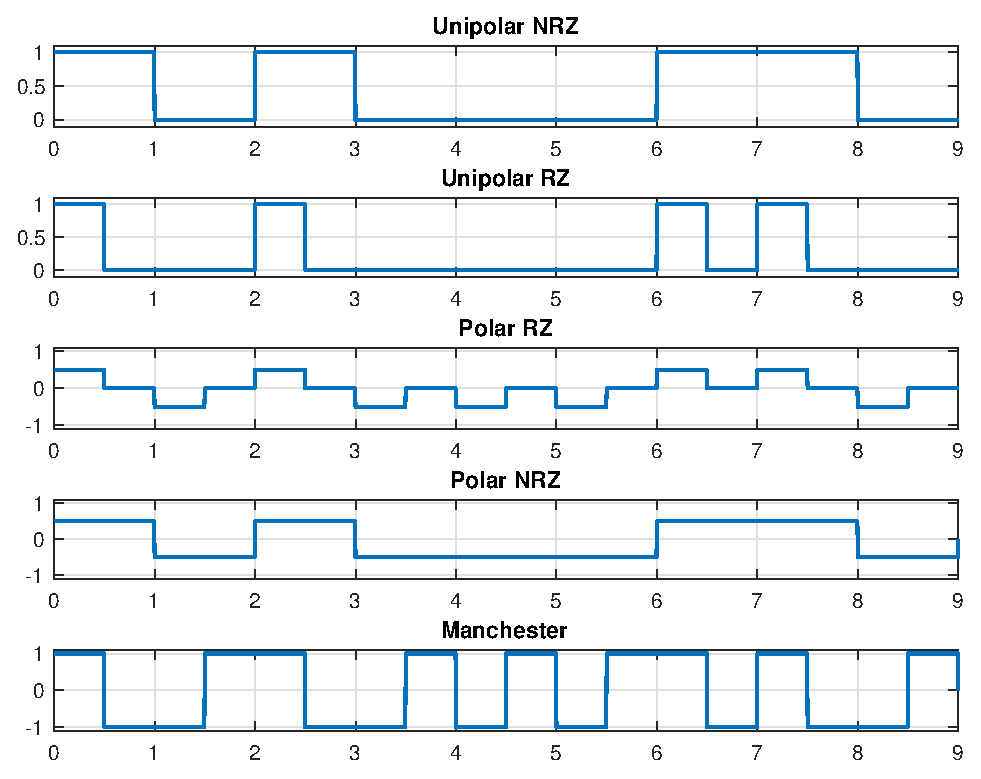
\includegraphics [width=4in]{Q8_01.eps}



\end{document}

